{\bf \large The material of this chapter is specific to the Windows 64-bit version of STEPSS, to its Java-based Graphic User Interface (GUI) and the Intel oneAPI Fortran Compiler. 

Before going any further, you have to read and accept the legal terms detailed at the beginning of this document.}

All needed files can be downloaded from the following \hypertarget{Google}{Google drive}:\\
\hspace*{-7ex}{\tt https://drive.google.com/drive/folders/1HcUSD-FOx6192HURJnxltYJuKuNA8Vwz?usp=drive\_link}

{\bf \large Note that the Java, Visual Studio and OneAPI files are not part of STEPSS}. They are provided only to ease the installation procedure, avoiding navigation through the Oracle, Windows and Intel Web pages.

%------------------------------------------------------------------------------------------------------
\section{Installing JAVA}


STEPSS comes with a Java-based Graphical User Interface (GUI). Everything is packed in a Java archive containing a (legal) copy of all executables and libraries required to run the simulations and display the results.

Using that GUI requires to have Java Version 20 installed on your computer. To check if you have Java installed, and if so, which version it is:
\begin{enumerate}
\item open a Windows Command prompt
\item in the latter, enter the command:\\
\hspace*{5ex}{\tt java -version}

It should display a message similar to the one shown in Fig.~\ref{fig_install_java}.
\item close the command prompt.
\end{enumerate}

\begin{figure}[h!]
\centering
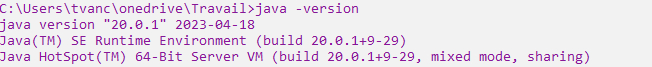
\includegraphics[scale=0.8]{java_check.jpg}
\caption{Checking the presence of the Java environment}\label{fig_install_java}
\end{figure}


If you have a previous version installed on your computer, it must be uninstalled following the standard Windows procedure:
\begin{enumerate}
\item click on Parameters
\item select Applications
\item locate Java
\item click on uninstall.
\end{enumerate}

Then, install Java Version 20 as follows:
\begin{enumerate}
\item download the Java SE Development Kit Version 20 (for 64-bit) from the \hyperlink{Google}{Google drive}. The 164-MB file is named {\tt jdk-20\_windows-x64\_bin.exe}
\item install by double-clicking on that file and following the instructions
\item for an easy execution, associate stepss.jar with Java following the standard Windows procedure:
\begin{enumerate}
\item right-click on the stepss.jar icon
\item select open with
\item choose always use this application.
\end{enumerate}
\end{enumerate}
   
Apart from the Java machine, STEPSS does not require any installation in the usual meaning of the term.
Just download the {\tt STEPSS.jar} file from the \hyperlink{Google}{Google drive} and drop it in any convenient place of the computer. The Windows desktop is a very convenient location.

Leave the archive intact; in particular do not uncompress it !  

STEPSS is launched by merely double-clicking on {\tt STEPSS.jar} (or a shortcut to the latter). 

When STEPSS is launched it creates a temporary working folder and copies all needed executables and libraries into that folder.

To remove STEPSS from your computer, just delete the archive file. STEPSS does not leave anything in your computer !

%--------------------------------------------------------------------------------------------------------
\section{Installing Visual Studio}

{\bf \large This step can be skipped if you do not plan to develop new models for RAMSES}.

The Intel OneAPI compiler relies on the Microsoft Visual Studio environnement as well as some associated C++ libraries.

The Community 2022 version is required. If you have a previous version installed on your computer, it must be uninstalled following the standard Windows procedure.

The installation steps are as follows:
\begin{enumerate}
\item download from the \hyperlink{Google}{Google drive} the launcher named\\
{\tt vs\_community\_\_e942d3d4864d4a80b72975352289d007.exe}
\item execute by double-clicking
\item during the installation, under the ``Workloads'' view, select the checkbox to install the ``Desktop development with C++'' component of Visual Studio as shown in Fig.~\ref{fig_Visual_Studio}. This component is not installed by default.
\end{enumerate}

\begin{figure}[h!]
\centering
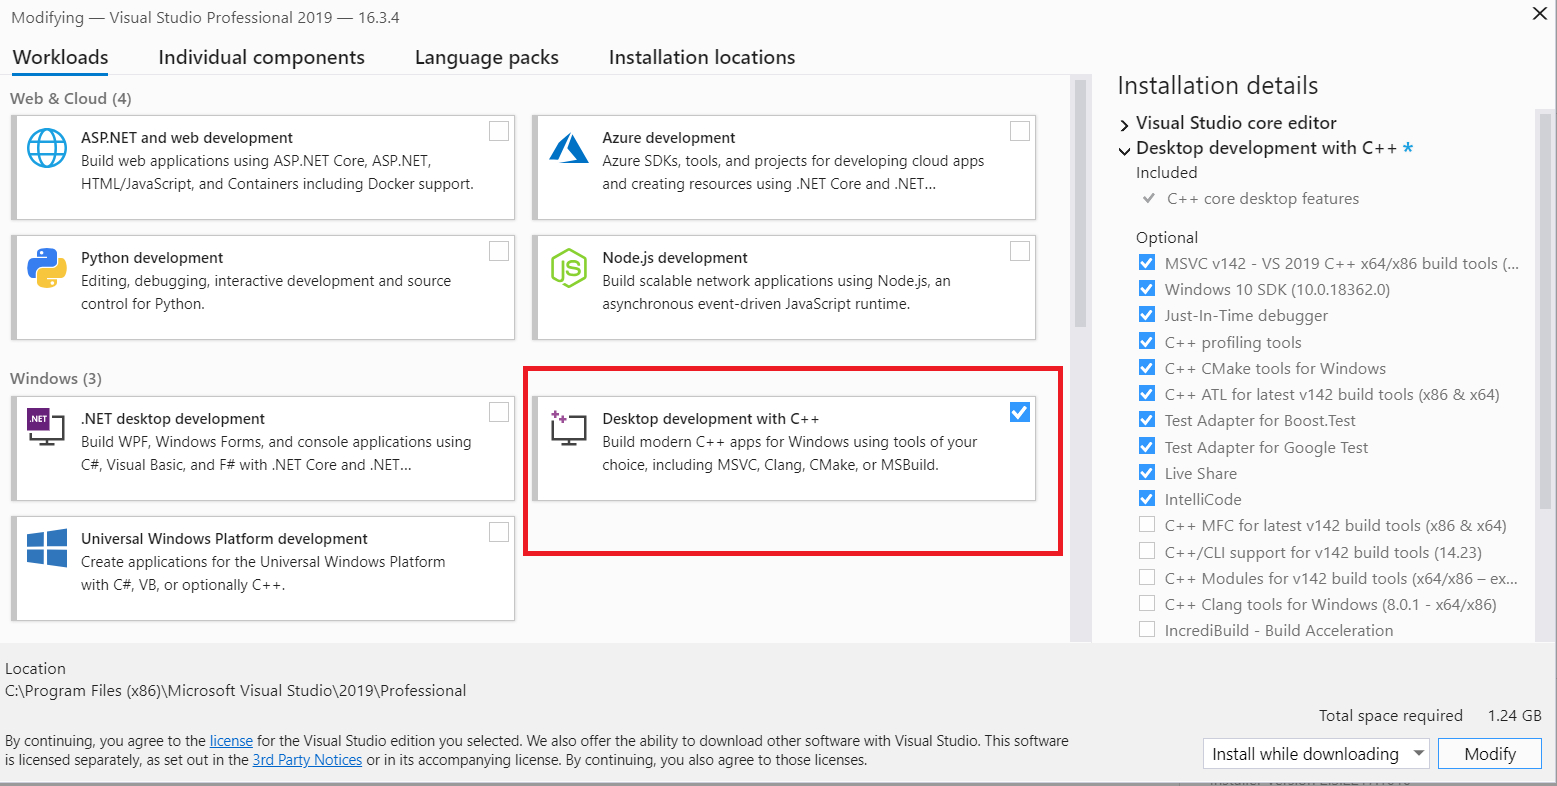
\includegraphics[scale=0.3]{Visual_Studio.jpg}
\caption{Selecting the ``Desktop development with C++'' component when installing Visual Studio}\label{fig_Visual_Studio}
\end{figure}
 
%--------------------------------------------------------------------------------------------------------
\section{Installing the Fortran Compiler}

{\bf This step can be skipped if you do not plan to develop new models for RAMSES}.

There are three packages to download and install.

\begin{enumerate}
\item download from the \hyperlink{Google}{Google drive} the OneApi Basekit. The file is named:\\
\hspace{5ex}{\tt w\_BaseKit\_p\_2023.1.0.47256\_offline.exe}
\item download from the \hyperlink{Google}{Google drive} the Fortran Compiler Classic package. The file is named:\\
\hspace{5ex}{\tt w\_ifort\_runtime\_p\_2023.1.0.46319.exe}
\item download from the \hyperlink{Google}{Google drive} the HPC toolkit. The file is named:\\
\hspace{5ex}{\tt w\_HPCKit\_p\_2023.1.0.46357\_offline.exe}
\item install each of the three packages, in the above order, by double-clicking on the .exe files
\item restart your computer.
\end{enumerate}




